\section{Path Server}
The \ISDC \PS maintains a path database that contains all $k$ paths registered by \STUB \ADs, and provide down-path resolution service to support \AD-level end-to-end path establishment.

\begin{figure*}[ht]
\centering
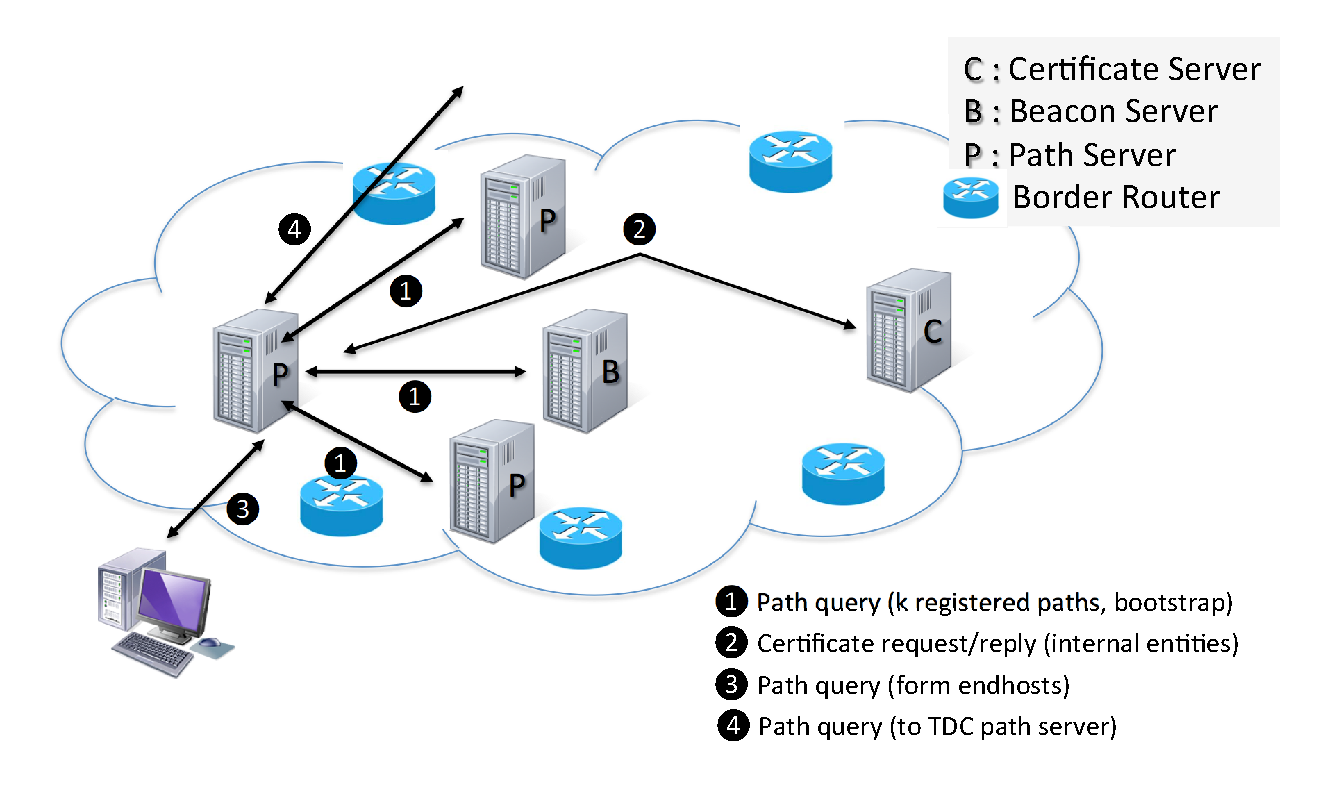
\includegraphics[width=.9\columnwidth]{./fig/ps_message.eps}
\caption{Path Server messages.}\label{fig:ps-message}
\end{figure*}

\subsection{Path Registration}
An \STUB \AD's path registration request includes the following information.
\begin{itemize}
\item {CTime: } Current time 
\item {AID: } ID of the requesting \AD %\newline
\item {Type: } [Public/Private], [Internal/External] %\newline
\item {Timestamp: } \ISDC's timestamp that shows the PCB initiation time 
%\item {Expiration Time: } Lifetime of the path. (Currently, we define 4 lifetimes: 6 hours, 12 hours, 18 hours, and 24 hours; viz., Figure~\ref{fig:hdr-common})
\item {Hops: } The number of \ADs (i.e., \AD hops) from \ISDC to the \STUB \AD
\item {PCB Header: } A series of AIDs and corresponding Opaque Fields (viz., Figure~\ref{fig:hdr-beacon}) %\newline
\item {Signature: } The requesting \AD's signature computed over the registration request information %\newline
\end{itemize}

\noindent The current time (CTime) is added to prevent replay attacks. The {\em Type} field determines the scope of path disclosure and is defined as follows. %\newline
\begin{itemize}
\item {Public (TYPE\_PUB): } A public path is used by all \ADs. %\newline
\item {Private (TYPE\_PRI): } A private path is encrypted with a secret key. This path can be used by the \ADs that know the secret key and hence decrypt the path information. %\newline
\item {Internal (TYPE\_INT): } An internal path is disclosed to the \ADs inside the ISD %\newline
\item {External (TYPE\_EXT): } An external path is disclosed to all \ADs outside the ISD %\newline
\end{itemize}

The \ISDC path server, on receiving an \AD's path registration request, verifies the signature in the request, and if the signature is correct, it replaces the \AD's oldest entry with the new path. If the path registration fails, the path server returns an error code. Possible error code includes:

\begin{itemize}
\item Unidentified \AD (including missing \AD certificate)
\item Signature verification failure
\item Maximum number of updates exceeded
\end{itemize}

Note that path registration is made to the path server in the \ISDC.

\subsection{Path Resolution} 
\STUB \ADs use the registered $k$ paths to the \ISDC for up-paths and down-paths ($k$ up-paths and $k$ down-paths can be different). A source \AD, in order to know how to reach the destination \AD (we assume that the sender (host) knows the AID of the destination \AD that hosts the receiver (host), using a DNS service), sends a path query to the \ISDC path server. The \ISDC \PS's response includes $k$ down-paths to the destination \AD, where each down-path is a series of ADs and their Opaque Fields. Then, the source \AD selects a down-path and constructs an end-to-end path by composing one of its up-path and the selected down-path.

To perform the above path resolution, the \ISDC \PS and local \PS should provide the following functions.

\noindent {\bf \ISDC \PS: } The \ISDC \PS, on receiving a path query, determines which paths to return using the AID and Type in the packet. If the server has the corresponding paths to the query, it sends paths to the requesting \AD. The query response is signed by the \ISDC \PS. \soobum{needs discussion. Signature on the query response is necessary for security, yet would introduce overhead to the \PS.} The \ISDC would have multiple \PSs for load balancing and replication. A Distributed Hash Table (DHT) would be a good practical candidate for distributed \PS implementation. \soobum{do we need to elaborate this?}


\noindent {\bf Local \AD \PS: } Local \PSs resolve both up-paths and down-paths for endhosts. For up-path resolution, a local \PS keeps the list of paths offered by the \BS in the same \AD. The \BS, whenever it receives a new path (i.e., PCB) to \ISDC,  multicasts the path to all \PSs inside the \AD. That, a local \PS is a passive server. However, the \PS, on its first wake-up, pulls the registered up-paths to \ISDC from other \PSs within the \AD; or the server pulls those paths from \ISDC (note that un-registered, low-priority up-paths are multicast to \PSs continuously). An endhost set AID to TDC for an up-path query. For down-path service, a local \PS send a path query to the \ISDC on behalf of an endhost and forward the response from the \ISDC to the endhost. Furthermore, the local \PS stores the query response in its local cache to promptly handle the same path request from other endhosts. Down-path caching help reduce path resolution latency and prevent frequent path requests to \ISDC that would overload the \ISDC \PSs.



\subsection{Path Database}
For path resolution services, \PSs maintains the following database.

\noindent {\bf \ISDC \PS: } Down-paths to \STUB \ADs inside the \ISD. \newline
A record of an \STUB \AD consists of the path registration information shown above.

\noindent {\bf Local \PS: } Up-paths to \ISDC and down-paths to remote \STUB \ADs.
A record of an up-path has the same format as that of down-paths, yet it ends with a \ISDC \AD instead of an \STUB \AD. The local \PS cache has the same data structure as that of the \ISDC \PS.

\subsection{Bootstrapping}
The \ISDC \PS are assumed to be highly replicated and synchronized. Hence, when a \PS starts and finds any other \PSs in the topology file (that is kept locally or retrieved from the \CS), the \PS synchronizes its database with those of other \PSs. Bootstrapping procedure may differ how \PS database is implemented (e.g., RDB, DHT). Currently, the \PS stores the snapshot of path database as a file periodically (in every 10 minutes). Local \PSs works similarly, yet they only synchronize up-paths (or at least registered $k$ up-paths, which can be retrieved from the \BS if the \AD has a single \PS) to \ISDC. Cached down-paths to remote \ADs are not required to be synchronized. 



